% Import Packages
\documentclass[12pt,a4paper]{article}
\usepackage[utf8]{inputenc}
\usepackage{amsmath,amsfonts,amssymb} %math related
\usepackage{fancyhdr} %fancy headers
\pagestyle{fancy} %something to do with page layout
\usepackage{float} %control over positions of figures etc
\usepackage{graphicx} %importing graphics
\usepackage{hyperref} %refrencing
\usepackage{relsize} %text changing sizes
\usepackage{tabularx} %table controls
%\usepackage{times} %times new roman font
\usepackage{titling} %fancy titles
\newcommand{\textsub}{\textsubscript}
% make command for \subtitle
\newcommand{\subtitle}[1]{%
  \posttitle{%
    \par\end{center}
    \begin{center}\large#1\end{center}
    \vskip0.4em}%
}


\date{September 9, 2019}

%Title Page
\title{WTFpga?}
\author{{Developed by Joe FitzPatrick} \\
		{FOSSified by Piotr Esden-Tempski and Clifford Wolf}\\
		{Presented by Josh Johnson}} 


%set margins
\usepackage[left=2cm,right=2cm,top=2.5cm,bottom=2.5cm,headheight=1cm]{geometry}
\fancyheadoffset{0cm}
\lhead{WTFpga?}
\chead{}
\rhead{}
\lfoot{}
\cfoot{}
\rfoot{\thepage}
\renewcommand{\headrulewidth}{0.4pt}

\begin{document}
%Title Page
\begin{titlingpage}
    \maketitle
\end{titlingpage}

\newpage

\section{Introduction}
Welcome to the workshop! This is a hands-on crash-course in Verilog and FPGAs in general. It is self-guided and self-paced. Josh is here to answer questions, not drone on with text-laden slides like usual.

While microcontrollers run code, FPGAs let you define wires that connect things together, as well as logic that continuously combines and manipulates the values carried by those wires. Verilog is a hardware description language
that lets you define how the FPGA should work. 

Because of this, FPGAs are well suited to timing-precise or massively-parallel tasks. If you need to repeatedly process a consistent amount of data with minimal delay, an FPGA would be a good choice. Signal and graphics processing problems, often done with GPUs if power and cost are no object, are often easy to parallelize and FPGAs allow you to widen your pipeline until you run out of resources. As your processing becomes more complicated, or your data becomes more variable, microcontrollers can become a
better solution.

The objective of this workshop is to do something cool with FPGAs in only two hours. In order to introduce such a huge topic in such a short time, LOTS of details will be glossed over. Two hours from now you’re likely to have more questions about FPGAs than when you started - but at least you’ll know the important questions to ask if you choose to learn more.

\section{What We Won't Learn}
In order to introduce Verilog and FPGAs in such a short time, we’re going to skip over several things that will be important when you build your own FPGA-based designs, but are not necessary to kickstart your tinkering: 
\begin{itemize}
	\item Synchronous Logic: We’re dealing entirely with human (AKA slow) input and output today. Running at maximum performance requires synchronizing all of the logic using a common clock, and optimizing the logic to fit that enforced timing.
	\item IP Cores: FPGA vendors pre-build or automatically generate code to let you easily interface your FPGA to interfaces like RAM, network, or PCIe. We’ll stick to LEDs and switches today.
	\item Simulation: Didn’t work right the first time? Simulation lets you look at all the signals in your design without having to use hardware or potentially expensive observation equipment.
	\item Testbenches: For effective simulation, you need to write even more Verilog code to stimulate the inputs to your system.
\end{itemize}

\newpage
\section{Meet the Hardware}
We will be using the not creatively named iCE40-feather board for this workshop. It contains an iCE40UP5K FPGA, USB programmer and USB to UART converter, LiPo battery charge control, and plenty of LEDs in an Adafruit Feather compatible form factor. To extend its capabilities for this workshop, we will be attaching a FeatherWing which has a dual seven segment display, eight DIP switches, and a slide switch. 

\begin{figure}[H]
\begin{centering}
	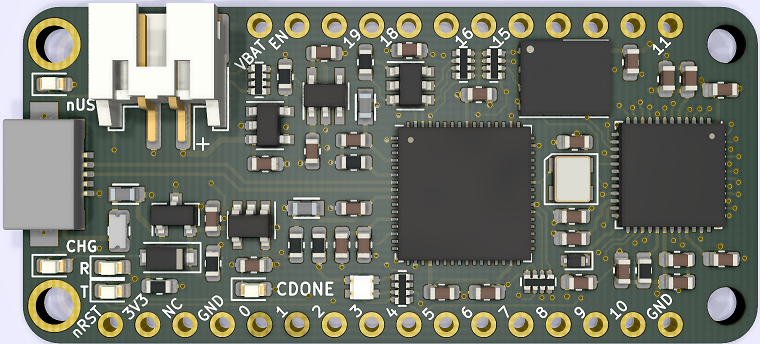
\includegraphics[width=\linewidth]{top_render.PNG}
	\caption{The iCE40-feather FPGA board being utilised.}
\end{centering}
\end{figure}

\begin{figure}[H]
\begin{centering}
	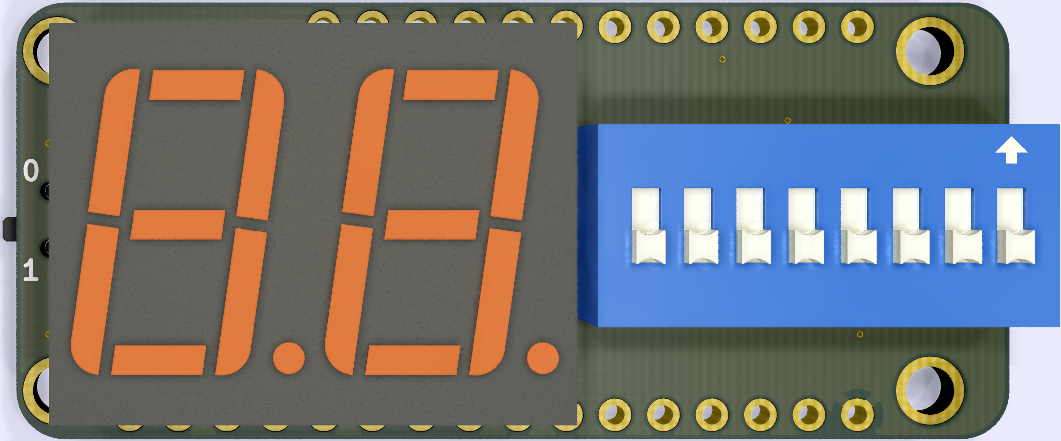
\includegraphics[width=\linewidth]{7segment_render.PNG}
	\caption{The seven segment and DIP switch FeatherWing.}
\end{centering}
\end{figure}
\newpage
\section{Getting to Blinky}
Due to time constraints, it is suggested that you install the toolchain and get a blinking LED on your iCE40-feather before attending the workshop. If you have not already installed the required yosys, nextpnr, and IceStorm tools, follow the instructions in \texttt{install.md}. If you do not have the FPGA dev board, read the instructions in \texttt{README.md} or get in contact with Josh. \\

\noindent
With the toolchain installed and hardware in hand, it is now time to blink some LEDs! If you have not already done so, clone the repository and open the blink directory.\\

\noindent
\textbf{git clone https://github.com/joshajohnson/WTFpga} \\
\textbf{cd WTFpga/blink}\\

\noindent
Now its time to walk through the process of synthesizing an FPGA design of your own and uploading it to the FPGA. We will be using the amazing open source tools called IceStorm, nextpnr and yosys. 
\begin{itemize}
		\item Ensure that the FPGA is connected via a USB cable to your computer. 
		\item Open the command line in the \textbf{WTFpga/blink} folder.
		\item Build and upload the gateware by typing \textbf{make prog} into the terminal. 
			\begin{itemize}
				\item NOTE: Windows users may need to run \textbf{make prog} twice due to path issues with the iceprog execuitable. 
			\end{itemize}
		\item Ensure that the led marked nUSR is blinking. If not it's time to begin troubleshooting!
			\begin{itemize}
				\item NOTE: Windows users may need to update drivers used with the FTDI IC used for USB to Serial communications. Check the install notes in \texttt{install.md}.
			\end{itemize}
		\item Once you get the LED blinking, open the file \texttt{blink.v} and have a look around. See if you can change the frequency of the blinking LED by altering the code. 
		\item After changing \texttt{blink.v} and saving it, run \textbf{make prog} again and confirm the frequency changes. 
\end{itemize}
If you have made it this far, congratulations! You have successfully programmed your FPGA, and can now attend the WTFpga workshop knowing that you'll hit the ground running. If you are having issues programming the board, get in contact with Josh and he will lend a hand troubleshooting. 
\newpage
\section{Reading Verilog}
Now that we know how to use the tools to configure our FPGA, let’s start by examining some simple Verilog code. Programming languages give you different ways of storing and passing data between blocks of code. Hardware Description Languages (HDLs) allow you to write code that defines how things are connected. 

\begin{itemize}
	\item \textbf{cd} to the directory \textbf{wtfpga-lab} and open \textbf{wtfpga.v} in the text editor of your choosing.
	\item Our module definition comes first, and defines all the inputs and outputs to our system. Can you locate them on your board?
	\item Next are wire definitions. Wires are used to	directly connect inputs to one or more outputs.
	\item Next are parallel assign statements, all of these assignments are always happening, concurrently. 
	\item In some designs, we would find always blocks. These are blocks of statements that happen sequentially, and are triggered by the sensitivity list contained in the following @(). We will run into them later in the lab.
	\item Finally we can instantiate modules. There are a few already instantiated but not really used for anything yet.
\end{itemize}
\noindent
Now let’s try and map our board’s functionality to the Verilog that makes it happen.
\begin{itemize}
	\item From the terminal we have open in the wtfpga-lab directory, type \textbf{make prog} and press enter to load the wtfpga project onto the FPGA. Windows users, remember you may have to run \textbf{make prog} twice due to the joys of iceprog. 
	\item What happenes when you move the DIP switches?
	\item Can you find the DIP switches in the module definition? What are they named?
	\item Can you find the assignments which use each of the switches? What are they assigned to?
	\item Can you follow the assignments to an output?
	\item Do you notice anything interesting about the order of the assign statements?
\end{itemize}
\noindent
You should be able to trace the DIP switches inputs, through a number of wires, to seven segment outputs. You should also note that the seven segment display is inverted, the reasoning of which will be explained later. 

Note that these aren't sequential commands. All of these things happen at once. It dosen't actually matter what order the assgn statements occur. 
\newpage
\section{Making Assignments}
Let’s start with some minor changes to our Verilog.
\begin{itemize}
	\item Remove all of the \textbf{assign seg[x] = sw[x];} assignments from the file 
	\item Replace the previous assignments with \textbf{assign seg[6:0] = $\sim$sw[6:0];}
\end{itemize}
\noindent
Next, we need to create a new configuration for our FPGA. Brace yourself - it will be really quick!
\begin{itemize}
	\item In the command line terminal that we opened earlier, type \textbf{make prog}, and press enter. 
\end{itemize}
\noindent
You should see some text scroll by and the new design should be uploaded and running within a few seconds. If we were using proprietary tools (Vivado or Quartus) as we did in V1 and V2 of this workshop, the synthesis would take approximately 8 minutes depending on the computer used. We used these 8 minutes to talk about the synthesis process itself. Even though we don’t have to wait that long, let’s talk what the software is doing and what tools are used to accomplish those steps. It is a bit different from a software compiler.

\begin{itemize}
	\item First, the software will synthesize the design - turn the Verilog code into basic logical blocks, optimizing it in the process using yosys. (http://www.clifford.at/yosys/)
	\item Next, the tools will implement the design. This takes the optimized list of registers and assignments, and places them into the logical blocks available on the specific FPGA we have configured, then routes the connections between them using the tool called nextpnr. (https://github.com/yosysHQ/nextpnr)
	\item When that completes, the fully laid out 	implementation needs to be packaged into a 	format for programming the FPGA. There are a 	number of options, but we will use a .bit bitstream file for programming over SPI using icepack from the IceStorm tool collection.
	(http://www.clifford.at/icestorm/)
	\item Hopefully everything will go as planned. If you have issues, look in the console for possible build errors. If you have trouble, ask for help!
	\item Finally, the .bin file needs to be sent to the FPGA over USB. When this happens, the existing configuration will be cleared and the new design will take its place using the iceprog tool.
\end{itemize}
\noindent
Check what happens when you move the DIP switches. Does it function as you expect? What has changed from last time?

\begin{itemize}
	\item Before continuing, remove the \textbf{assign anode = 2'b11;} and \textbf{assign seg[6:0] = $\sim$sw[6:0];} statements from your design, and comment in the \textbf{displayMux} module. 
\end{itemize}

\newpage
\section{Combinational Logic}
Simple assignments demonstrate the parallel nature of FPGAs, but combinational logic makes it much more useful. We’re going to write a small module (like a procedure) that will convert the binary value shown on the DIP switches into a hex digit on the 7-segment display.

\begin{figure}[H]
	\begin{centering}
		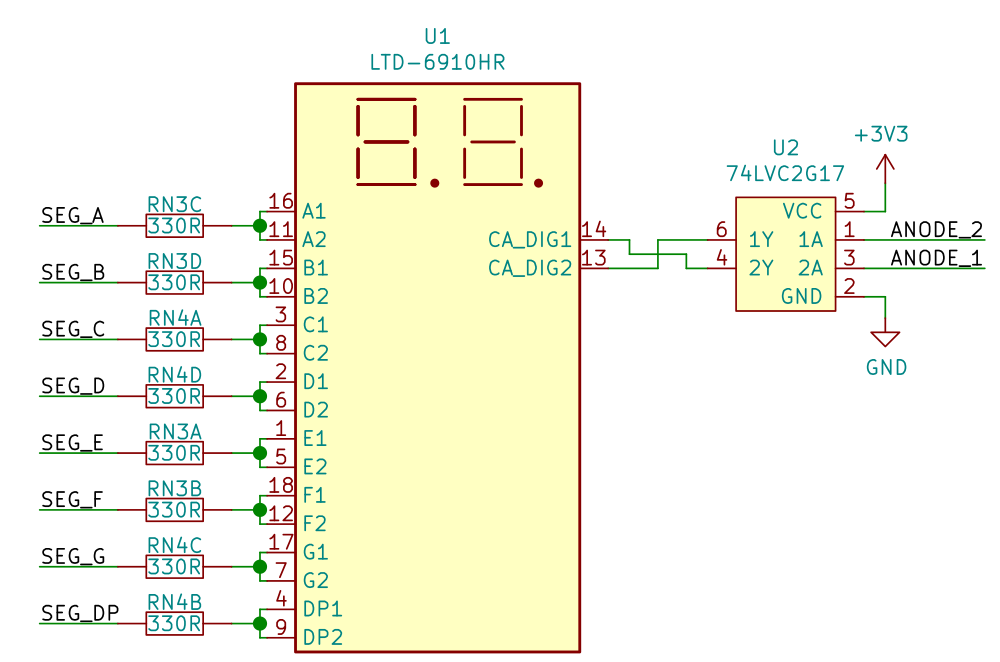
\includegraphics[width=\linewidth]{sevenSeg.png}
		\caption{Schematic for the seven segment display.}
	\end{centering}
\end{figure}
\noindent
There are 7 \textbf{seg} output wires that control which LEDs are on or off, and correspond from \textbf{A} to \textbf{G} on the display. There are two anode wires connected through buffers to select which digit is on, and corresponds to \textbf{CA\_DIG1} and \textbf{CA\_DIG2} on the right. To display two different characters, we need to cycle between them fast enough so that they persist in the eye. All of the code to generate the clock (clockDiv.v) and multiplex the display (dispMux.v) is already written and included in the project, giving direct access to each of the displays as disp0 and disp1.

\begin{itemize}
	\item First, let's connect the stubbed-out \textbf{nibbleDecode} module into our design. 
	\begin{itemize}
		\item Find \textbf{nibbleDecode} in \textbf{wtfpga.v}. The module is instanticated, but not connected to anything. 
		\item Connect the low 4 bits of our switches to the nibblein field: \textbf{.nibblein(sw[3:0]),}
		\item Connect the 7 bits of output to the right most seven segement display: \textbf{.seg(disp1)}
	\end{itemize}
	\item Next, let's duplicate it so we can see a full hex byte.
	\begin{itemize}
		\item Copy and paste a new \textbf{nibbleDecode} instantiation. 
		\item Rename it from \textbf{nibbleDecodeLSD} to \textbf{nibbleDecodeMSD} as this will display the most significant digit (left most display).
		\item Connect the upper 4 bits of the switches \textbf{sw[7:4]} to \textbf{nibblein}, and rename the output display to \textbf{disp0}.
	\end{itemize}
	\item We now need to implement logic which converts our binary value into a character on the seven segement display.
	\begin{itemize}
		\item Open \textbf{nibbleDecode.v} in your text editor. 
		\item We're going to use a case statement to convert a binary nibble into a series of bits which represent the seven segment display segements which need to be illuminated. 
		\item For each case, we need the expected value of \textbf{nibbleIn}, and the correct value of \textbf{seg}, an array of bits which represent the segments on the display shown below.
		\begin{figure}[H]
		\begin{center}
			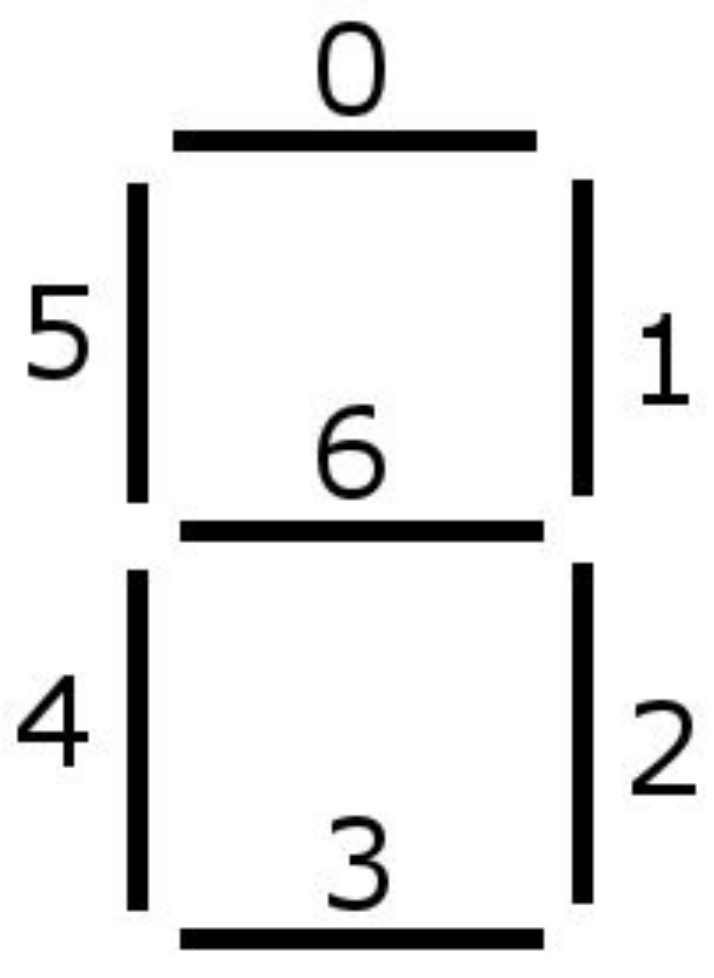
\includegraphics[width=0.25\linewidth]{segments.png}
			\caption{Mapping of seven segment segments to position. Typically labeled A through G.}
		\end{center} 
	\end{figure}
		\item Due to the display using a common anode, when a bit is '0', the corresponding segment is ON, and when a bit is a '1' the segment is OFF. Since that is confusing, we can use the $\sim$ operator for bitwise inversion such that '1' means the segment is illuminated. 
		\item For example, hex '1' looks like \textbf{$\sim$7'b0000110}. We can express this as \\ \textbf{4'h1: seg = $\sim$7'b0000110}, which roughly translates to:
		\begin{table}[H]
			\centering
			\begin{tabular}{lllll}
				\textbf{4'}        & when our 4 bits          &  &  &  \\
				\textbf{h1:}       & equal hex 0x01           &  &  &  \\
				\textbf{seg =}   & assign a value to seg    &  &  &  \\
				\textbf{$\sim$7'b} & of seven inverted bits   &  &  &  \\
				\textbf{0000110}   & leds 1 and 2 illuminated &  &  & 
			\end{tabular}
		\end{table}
		\item Figure out what you need to set for the remaining hex values using the diagram. 
	\end{itemize}
	\item Due to how included files are handled in this lab, you will have to \textbf{make clean} before running \textbf{make prog} after editing a file other than \textbf{wtfpga.v}.
	\item \textbf{make clean} then \textbf{make prog} your design. Does it work?
\end{itemize}
\section{Registers}
While there is so much more to combinatorial logic than we actually touched on, let's move on to a new concept - registers. Assignments are excellent at connecting blocks together, but they're more similar to pass paramaters than actual variables. Registers allow you to capture and store data for repeated or later use. \\

\noindent
Whilst in previous editions of this workshop a calculator was implemented to demonstrate registers, due to the lack of buttons we will use registers to allow us to gracefully display decimal values on the seven segment display. Whilst this isn't the best demonstration of register use, it should hopefully give you an idea of how they can be utilised.

\begin{itemize}
	\item Open \textbf{wtfpga.v} in your text editor. 
	\item Un-comment the instantiation of \textbf{displaySelect}.
	\item We will use \textbf{displaySelect} to take the binary value of the DIP switches \textbf{sw}, along with the state of the \textbf{switch} on the left of the seven segment display, to output either decimal or hexadecimal values through \textbf{nibbleMS} and \textbf{nibbleLS} to display on the seven segment display. 
	\item Instead of connecting the switches directly to the decoders, we need to route them through the \textbf{displaySelect} module. 
	\item Define two \textbf{wires}, \textbf{nibbleMS} and \textbf{nibbleLS} of width \textbf{[3:0]} to act as intermediary signals.
	\item In the \textbf{nibbleDecode} modules, replace the \textbf{sw[3:0]} and \textbf{sw[7:4]} wires with \textbf{nibbleLS} and \textbf{nibbleMS}.	
\end{itemize} 

\noindent
Now we have an instantiation for \textbf{displaySelect}, we need to add some logic for it to be useful.
\begin{itemize}
	\item Open \textbf{displaySelect.v} in your text editor. 
	\item Find the \textbf{always @} block.
	\begin{itemize}
		\item \textbf{always @} is the header for a synchronous block of code.
		\item The list in parenthesis following \textbf{@} is the \textbf{Sensitivity List}. Whenever one of the signals in the sensitivity list changes, the block is run. It is similar to binding a callback function or mapping an interrupt in software terms. 
	\end{itemize} 
		\item Lets put \textbf{posedge clk} in the sensitivity list. This means each of positive edge - every time the \textbf{clk} goes from low to high - we will execute this block: \textbf{always @(posedge clk)}
		\item Now, we need to choose if we will display hexadecimal or decimal values depending on the state of \textbf{switch}. Add \textbf{switch} into the brackets of the if - else block. 
		\item When in hex mode, all we need to do is route the DIP switch (\textbf{sw}) wires out of the module and back to the decoder as before. This can be achieved by adding \\ \textbf{nibbleMS $<=$ sw[7:4];}, along with the corresponding line for the least significant nibble in the if block. Note that assignments are different inside the always block - we are setting a register, not assigning a wire anymore! 
		\begin{itemize}
			\item You may be wondering what that strange \textbf{$<=$} sign is, and why is isn't a \textbf{=} like you typically see in most programming languages?
			\item \textbf{$<=$} is a \textbf{non blocking} assignment, and means that in an always block, every line will be executed in parallel. 
			\item On the other hand, \textbf{=} is a \textbf{blocking} assignment, and ensures that the following line of code will only be executed after it's previous line has been executed. 
			\item We will cover this in more detail in next month's meetup.
		\end{itemize}
		\item Build this design with \textbf{make clean} then \textbf{make prog} and ensure it works so far. The display should function as normal when the switch is in the \textbf{1} position, but should be static when in the \textbf{0} position. 
	\end{itemize}
	To implement the decimal decoding, we need to determine what digit needs to be shown on each display. In software, a straightforward implementation would involve taking the number modulo 10 to find the digit in the ones position, and then subtracting that from the total number to find the value in the tens column.  However, division and modulo operations are computationally expensive, and for reasons we will not cover over should not be implemented on an FPGA though using the \textbf{/} and \textbf{\%} operators.
	
	Instead, we will use if else statements to determine the number in the tens column, and then subtract this from the total value to find the number to display in the ones position.  
	
	\begin{itemize}
		\item Uncomment the lines below "determine value to display in most significant display". It compares the number from the DIP switch to 90, 80, etc, and sets \textbf{nibbleMS} which is then displayed in the tens position. Complete the rest of the statements. 
		\item Complete the calculation of \textbf{nibbleLS} through inserting the correct values into the incomplete calculation. Hint: implement the sentence above these dot points.
		\item \textbf{make clean} then \textbf{make prog} to upload the updated gateware to the FPGA. Move the slide switch up into the \textbf{0} position and confirm that it decodes to decimal correctly. What happens when you count past 99? How can we solve this?
	\end{itemize}
	One method of resolving this would to not allow the displayed number to go above 99. Another would be to only show the two lowest digits on the display. I'll show you how to implement the former.
	\begin{itemize}
		\item First, below the module definition, instantiate a register of width 8 called dispNum which will hold the value displayed. You can do this, and set it's initial state to 0 with: \\ \textbf{reg [7:0] dispNum = 0;}
		\item Now, directly between the \textbf{end else begin} and \textbf{if (dispNum $\ge$ 7'd90) begin} lines, we need to add an if statement to do the following: \\ 
		\textbf{if (sw $\le$ 99) begin}\\
		set \textbf{dispNum} equal to \textbf{sw}\\
		\textbf{end else begin}\\
		set \textbf{dispNum} to \textbf{99}\\
		\textbf{end}
		\item Now change the \textbf{sw} variable to \textbf{dispNum} for all occurrences below this line.
		\item Run your code and confirm that it limits the display to 99. Now, by adding an additional if statement and some more logic, configure the display to only show the lowest two digits on the display when it runs out of space.
	\end{itemize}



\newpage
\section{Exploring More}
You've now completed the seven segment decoder, which uses most of the core concepts used to design nearly all silicon devices in use today. If time permits, there are a few additional things you can explore or try with this board. 
\begin{itemize}
	\item Examine the \textbf{feather.pcf} file. This contains all of the mappings of the FPGA's pins to the names you use in your code. 
	\item Examine \textbf{clkDiv.v} in your text editor. This is a clock divider that divides the 12MHz reference clock into lower speed clocks used internally. What does it do? How does it seem to work?
	\item Modify \textbf{clkDiv.v} to speed up or slow down the clock. What happens? 
	\item Modify the design to flash the LEDs.
	\item Modify the design to PWM fade the LEDs. 
	\item Modify \textbf{dispDecode.v} along with \textbf{wtfpga.v} to allow more than just hexadecimal numbers to be displayed.
	\item Examine the \textbf{displayMux.v} file. What does it do? How does it seem to work? Can you dim the display? 
	\item Turn the display into a countdown timer, wherein you set a number on the display, and then move the slide switch to begin the countdown. For even more of a challenge, once the timer has reached 0, flash the display.
	\item Have a chat to Josh about the design and assembly of the iCE40-feather and how FPGA implementation differs from microcontrollers. For those interested, the design files are available at \url{github.com/joshajohnson/iCE40-feather}, and additionally a PDF schematic is available in the \textbf{WTFpga/docs} folder.
\end{itemize}

\newpage
\section{Thank You and Further Resources}
I hoped you enjoyed this rather short dive into FPGA development. What's next? Over the next one or two (not sure yet!) meetups we will dive further into the world of FPGAs, and cover some of the topics we skipped, along with some of the questions I'm sure you have. \\

\noindent
If you have any comments, questions, or feedback, please either have a chat in person of get in contact through one of the following channels:\\
\noindent
Email: \texttt{josh@joshajohnson.com}\\
Twitter: \texttt{@\_joshajohnson}\\
BSidesCBR Slack: \texttt{josh}\\ 

\noindent
If you are looking for something to keep you entertained until next month, below are some resources which may be useful. \\

\noindent
Hamsterworks has a wiki full of many things to do with FPGAs including multi-part FPGA courses and projects: \url{http://hamsterworks.co.nz/mediawiki/index.php/Main_Page}\\

\noindent
ASIC World has a Verilog guide along with examples and references: \url{http://www.asic-world.com/verilog/veritut.html}\\

\noindent
nandland has a bunch of FPGA related content, along with a YouTube channel. \url{https://www.nandland.com/}\\

\noindent
The repo for the iCE40-feather contains more documentation regarding the board, along with a few example projects. I haven't had much time to design projects for it, so if you build something using the board please open a pull request with your design! \url{https://github.com/joshajohnson/iCE40-feather} \\

\noindent
Thanks once again for coming along, and I hope to see everyone here next month for even more FPGA fun!
\end{document}